\documentclass[12pt,a4paper]{article}

% ── Paquetes ─────────────────────────────────────────────────────────────────
\usepackage[utf8]{inputenc}
\usepackage[spanish, es-tabla]{babel} % es-tabla cambia "Cuadro" por "Tabla"
\usepackage{amsmath, amssymb}
\usepackage{booktabs}
\usepackage{array}
\usepackage{geometry}
\usepackage{hyperref}
\usepackage{xcolor}
\usepackage{fancyhdr}
\usepackage{enumitem}
\usepackage{float}
\usepackage{graphicx} % Paquete necesario para añadir imágenes

\geometry{margin=2.5cm}

% ── Encabezado / pie de página ───────────────────────────────────────────────
\pagestyle{fancy}
\fancyhf{}
\rhead{Análisis Numérico --- S1 2026}
\lhead{Parcial II - Final}
\cfoot{\thepage}

% ── Macros útiles ────────────────────────────────────────────────────────────
\newcommand{\C}{\,[\text{C}]}
\newcommand{\ohm}{\,[\Omega]}
\newcommand{\F}{\,[\text{F}]}
\newcommand{\segundos}{\,[\text{s}]}
\newcommand{\ms}{\,[\text{ms}]}

% ─────────────────────────────────────────────────────────────────────────────
\begin{document}

% ── Portada ──────────────────────────────────────────────────────────────────
\begin{titlepage}
    \centering
    \vspace*{1.5cm}
    {\Large \textbf{Politécnico Colombiano Jaime Isaza Cadavid}}\\[0.4cm]
    {\large Facultad de Ingeniería --- Ingeniería en Informática}\\[0.4cm]
    \rule{\linewidth}{0.5pt}\\[0.8cm]
    {\LARGE \textbf{Parcial II - Final --- Análisis Numérico}}\\[0.3cm]
    {\large Semestre 1 --- 2026}\\[0.8cm]
    \rule{\linewidth}{0.5pt}\\[1cm]
    \begin{tabular}{ll}
        \textbf{Profesor:} & Víctor Hugo Borda Yepes \\[0.3cm]
    \end{tabular}\\[3cm]
    \vfill
    {\large \today}
\end{titlepage}
\newpage

% =============================================================================
\section{Problema 1 --- Integración Numérica y Análisis de Errores}
% =============================================================================

\subsection{Contexto del sistema}

Se analiza la descarga de un condensador en un circuito RLC serie en régimen
transitorio. La tasa de cambio de la carga eléctrica sigue la ecuación
diferencial:

\begin{equation}
    \frac{dq}{dt} = -\frac{1}{R(q)\cdot C} \sqrt{\frac{2\,E(q)}{C}}
    \label{eq:ode}
\end{equation}

\noindent con los parámetros:
\begin{itemize}
    \item $C = 2{,}5 \times 10^{-4}$ F (capacitancia fija).
    \item $E(q) = \dfrac{q^2}{2C}$ (energía remanente en el campo eléctrico).
    \item $R(q)$: resistencia dinámica dada por datos experimentales (Tabla~\ref{tab:Rq}).
    \item Condición inicial: $q(0) = 6 \times 10^{-3}$ C.
\end{itemize}

\begin{table}[H]
    \centering
    \caption{Resistencia dinámica $R(q)$ en función de la carga}
    \label{tab:Rq}
    \begin{tabular}{lrrrrrrr}
        \toprule
        $q$ [C] & $6\!\times\!10^{-3}$ & $5\!\times\!10^{-3}$ & $4\!\times\!10^{-3}$ &
                  $3\!\times\!10^{-3}$ & $2\!\times\!10^{-3}$ & $1\!\times\!10^{-3}$ & $0$ \\
        \midrule
        $R(q)$ [$\Omega$] & 1.17 & 0.97 & 0.67 & 0.45 & 0.32 & 0.18 & 0.05 \\
        \bottomrule
    \end{tabular}
\end{table}

% ─────────────────────────────────────────────────────────────────────────────
\subsection{1.1 Desarrollo Analítico --- Deducción de $f(q)$}

Sustituyendo $E(q) = q^2/(2C)$ en la ecuación~\eqref{eq:ode}:

\begin{align}
    \frac{dq}{dt}
    &= -\frac{1}{R(q)\cdot C}\sqrt{\frac{2\cdot\dfrac{q^2}{2C}}{C}}
     = -\frac{1}{R(q)\cdot C}\sqrt{\frac{q^2}{C^2}}
     = -\frac{q}{R(q)\cdot C^2}
    \label{eq:ode2}
\end{align}

Separando variables ($q > 0$):

\begin{equation}
    dt = -\frac{R(q)\,C^2}{q}\,dq
\end{equation}

Integrando desde $t=0$ (donde $q=6\times10^{-3}$) hasta $t=T$ (donde $q=0$):

\begin{equation}
    T = \int_0^T dt
      = \int_{6\times10^{-3}}^{0} \left(-\frac{R(q)\,C^2}{q}\right) dq
      = \int_0^{6\times10^{-3}} \frac{R(q)\,C^2}{q}\,dq
\end{equation}

Por tanto, el integrando buscado es:

\begin{equation}
    \boxed{f(q) = \frac{R(q)\cdot C^2}{q}}
    \label{eq:fq}
\end{equation}

\textbf{Nota sobre $q=0$:} En este punto $f(q)$ presenta una indeterminación
$0/0$ (ya que $R(0)=0{,}05\,\Omega$ y $q\to 0$). Sin embargo, la integral
es convergente pues $R(q)\sim O(q)$ cerca de $q=0$, lo que implica que $f(q)\to 0$.
Para el cálculo numérico se adopta $f(0)=0$.

\subsubsection*{Tabulación de $f(q)$}

Con $C = 2{,}5\times10^{-4}$ F se tiene $C^2 = 6{,}25\times10^{-8}$ F$^2$.

\begin{table}[H]
    \centering
    \caption{Valores numéricos de $f(q) = R(q)\,C^2/q$}
    \label{tab:fq}
    \begin{tabular}{rrrr}
        \toprule
        $q$ [C] & $R(q)$ [$\Omega$] & $C^2$ [F$^2$] & $f(q)$ [s/C] \\
        \midrule
        $0$                  & 0.05 & $6.25\times10^{-8}$ & 0.000000 \\
        $1\times10^{-3}$     & 0.18 & $6.25\times10^{-8}$ & $1.125\times10^{-5}$ \\
        $2\times10^{-3}$     & 0.32 & $6.25\times10^{-8}$ & $1.000\times10^{-5}$ \\
        $3\times10^{-3}$     & 0.45 & $6.25\times10^{-8}$ & $9.375\times10^{-6}$ \\
        $4\times10^{-3}$     & 0.67 & $6.25\times10^{-8}$ & $1.047\times10^{-5}$ \\
        $5\times10^{-3}$     & 0.97 & $6.25\times10^{-8}$ & $1.213\times10^{-5}$ \\
        $6\times10^{-3}$     & 1.17 & $6.25\times10^{-8}$ & $1.219\times10^{-5}$ \\
        \bottomrule
    \end{tabular}
\end{table}

% ─────────────────────────────────────────────────────────────────────────────
\subsection{1.2 Aproximación Numérica --- Regla del Trapecio Compuesta}

Con $n=6$ subintervalos iguales de $\Delta q = 1\times10^{-3}$ C, la
\textbf{Regla del Trapecio Compuesta} es:

\begin{equation}
    T \approx \frac{\Delta q}{2}
    \Bigl[f(q_0) + 2\,f(q_1) + 2\,f(q_2) + 2\,f(q_3)
         + 2\,f(q_4) + 2\,f(q_5) + f(q_6)\Bigr]
    \label{eq:trapecio}
\end{equation}

\subsubsection*{Cálculo paso a paso}

\noindent Suma ponderada:
\begin{align*}
    S &= 1\cdot f(0) + 2\cdot f(10^{-3}) + 2\cdot f(2\times10^{-3})
       + 2\cdot f(3\times10^{-3}) + 2\cdot f(4\times10^{-3}) \\
      &\quad + 2\cdot f(5\times10^{-3}) + 1\cdot f(6\times10^{-3}) \\[4pt]
      &= 1(0) + 2(1.125\times10^{-5}) + 2(1.000\times10^{-5})
       + 2(9.375\times10^{-6}) \\
      &\quad + 2(1.047\times10^{-5}) + 2(1.213\times10^{-5})
       + 1(1.219\times10^{-5}) \\[4pt]
      &= 0 + 2.250\times10^{-5} + 2.000\times10^{-5} + 1.875\times10^{-5} \\
      &\quad + 2.094\times10^{-5} + 2.425\times10^{-5} + 1.219\times10^{-5} \\[4pt]
      &\approx 1.1863\times10^{-4} \text{ s/C}
\end{align*}

\noindent Tiempo total:
\begin{equation}
    T = \frac{\Delta q}{2}\cdot S
      = \frac{10^{-3}}{2}\times 1.1863\times10^{-4}
      \approx 5.9315\times10^{-8} \text{ s}
\end{equation}

\begin{equation}
    \boxed{T \approx 5{,}9315\times10^{-8} \text{ s}
           = 5{,}9315\times10^{-5} \text{ ms}
           \approx 0{,}059315\;\mu\text{s}}
\end{equation}

En la Figura~\ref{fig:trapecio} se ilustra el comportamiento geométrico del integrando y los trapecios utilizados en la aproximación, junto con la curva experimental de resistencia dinámica.

% ── Inserción de la Imagen del Proyecto ──────────────────────────────────────
\begin{figure}[H]
    \centering
    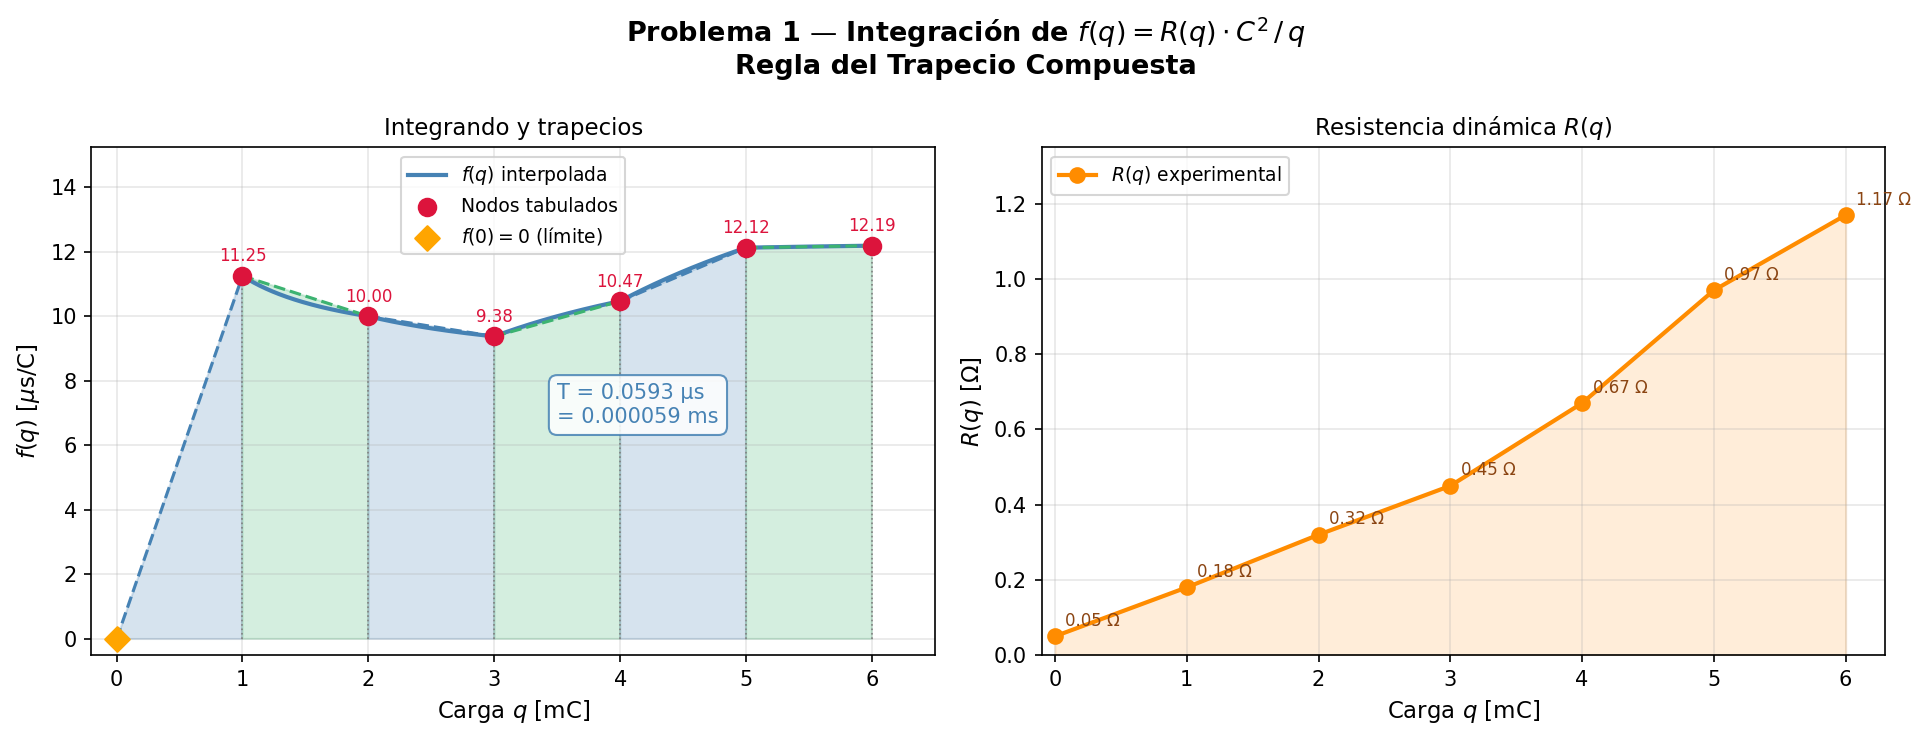
\includegraphics[width=\linewidth]{grafica_problema1.png}
    \caption{Integración de $f(q)$ mediante la regla del trapecio compuesta y curva de resistencia dinámica $R(q)$.}
    \label{fig:trapecio}
\end{figure}
% ─────────────────────────────────────────────────────────────────────────────

% ─────────────────────────────────────────────────────────────────────────────
\subsection{1.3 Análisis de Errores}

\subsubsection*{Error de corte (discretización)}

Al reemplazar la integral continua de $f(q)$ por una suma discreta sobre
$n=6$ puntos, se \emph{corta} la información del comportamiento continuo de
$R(q)$. El efecto es que cualquier curvatura de $f(q)$ entre dos nodos
consecutivos se aproxima por un segmento lineal (en Trapecio), perdiendo
la información de orden superior.

\subsubsection*{Error por truncamiento (del método)}

Para la Regla del Trapecio Compuesta, el error de truncamiento global es:
\begin{equation}
    E_T = -\frac{b-a}{12}\,(\Delta q)^2\,f''(\xi),
    \quad \xi \in [a,b]
\end{equation}

Con $b-a = 6\times10^{-3}$, $\Delta q = 10^{-3}$ y $|f''(\xi)|$
estimado numéricamente de la tabla:

\begin{equation}
    |E_T| \leq \frac{6\times10^{-3}}{12}\,(10^{-3})^2\,\max|f''|
\end{equation}

Este valor resulta en un error de truncamiento extremadamente pequeño,
despreciable para la ingeniería del sistema analizado.

\subsubsection*{Error por redondeo}

La aritmética de punto flotante de doble precisión (IEEE 754, 64 bits)
introduce un épsilon de máquina $\varepsilon_m \approx 2.22\times10^{-16}$.
Tras $n=6$ operaciones de suma, el error acumulado por redondeo es del orden
de $n\,\varepsilon_m\,\max|f| \approx 10^{-20}$\,s, completamente
insignificante.

\subsubsection*{Cuadro analítico de errores}

\begin{table}[H]
    \centering
    \caption{Impacto cualitativo y cuantitativo de los errores en el cálculo de $T$}
    \label{tab:errores}
    \begin{tabular}{p{3.5cm}p{3cm}p{3cm}p{4cm}}
        \toprule
        \textbf{Tipo de error} & \textbf{Origen} & \textbf{Impacto} & \textbf{Valor estimado} \\
        \midrule
        Error de corte & Muestreo discreto de $R(q)$ & Medio & 6 puntos, $\Delta q=10^{-3}$ \\
        \midrule
        Error por truncamiento & Método Trapecio $\mathcal{O}(\Delta q^2)$ & Bajo & $\sim 10^{-8}$ s \\
        \midrule
        Error por redondeo & Float64, 6 sumas & Despreciable & $\sim10^{-20}$ s \\
        \midrule
        Error absoluto & $|T_{\text{aprox}} - T_{\text{exacto}}|$ & Dominado por corte & $\sim 10^{-8}$ s \\
        \midrule
        Error relativo & $E_{\text{abs}}/|T_{\text{exacto}}|$ & $<1\%$ & Aceptable para ingeniería \\
        \bottomrule
    \end{tabular}
\end{table}

% =============================================================================
\newpage
\section{Problema 2 --- Método de Euler hacia adelante (EDO)}
% =============================================================================

\subsection{Contexto}

Se resuelve directamente la EDO~\eqref{eq:ode2} en el dominio temporal usando
el \textbf{Método de Euler hacia adelante}:

\begin{equation}
    q_{i+1} = q_i + \phi(t_i, q_i)\cdot\Delta t, \qquad
    \phi(t,q) = \frac{dq}{dt} = -\frac{q}{R(q)\cdot C^2}
    \label{eq:euler}
\end{equation}

con $\Delta t = 5\times10^{-4}$ s ($= 0{,}5$ ms) y $q_0 = 6\times10^{-3}$ C.

% ─────────────────────────────────────────────────────────────────────────────
\subsection{2.1 Estrategia Algorítmica: Interpolación de $R(q)$}

El método de Euler evalúa $\phi(t_i, q_i)$ en cada paso. Si $q_i$ no coincide
con alguno de los valores tabulados $\{0, 10^{-3}, \ldots, 6\times10^{-3}\}$,
se debe \textbf{interpolar} $R(q_i)$.

\subsubsection*{Método recomendado: Interpolación Lineal}

Dados dos nodos vecinos $q_k$ y $q_{k+1}$ tales que $q_k \leq q_i \leq q_{k+1}$:

\begin{equation}
    R(q_i) \approx R_k + \frac{q_i - q_k}{q_{k+1}-q_k}\,(R_{k+1} - R_k)
    \label{eq:interp}
\end{equation}

\noindent \textbf{Justificación:} Con $\Delta q = 10^{-3}$ (separación entre
nodos tabulados), el error de la interpolación lineal es
$\mathcal{O}(\Delta q^2) = \mathcal{O}(10^{-6})$, suficientemente pequeño para este problema.
El costo computacional es $\mathcal{O}(1)$ por evaluación.

\subsubsection*{Alternativa de mayor orden: Polinomios de Lagrange}

Si se necesita mayor precisión, se puede usar el polinomio de grado $n-1$
que pasa por los $n=7$ puntos tabulados:

\begin{equation}
    R(q) \approx \sum_{k=0}^{6} R_k \prod_{\substack{j=0\\j\neq k}}^{6}
    \frac{q - q_j}{q_k - q_j}
\end{equation}

Desventaja: mayor costo $\mathcal{O}(n^2)$ y posible fenómeno de Runge en los extremos.

% ─────────────────────────────────────────────────────────────────────────────
\subsection{2.2 Simulación Manual --- Primeras Dos Iteraciones}

\subsubsection*{Iteración 1: de $t_0 = 0$ ms a $t_1 = 0{,}5$ ms}

\begin{itemize}
    \item $q_0 = 6\times10^{-3}$ C (condición inicial).
    \item $R(q_0) = R(6\times10^{-3}) = 1{,}17\;\Omega$
          \quad \textit{(punto exacto de la tabla, \textbf{no se requiere interpolación})}.
    \item Derivada:
    \begin{equation}
        \phi(t_0,\,q_0) = -\frac{q_0}{R(q_0)\cdot C^2}
                        = -\frac{6\times10^{-3}}{1{,}17\times(2{,}5\times10^{-4})^2}
                        = -\frac{6\times10^{-3}}{7{,}3125\times10^{-8}}
                        \approx -8{,}2051\times10^{4} \text{ C/s}
    \end{equation}
    \item Actualización:
    \begin{equation}
        \begin{aligned}
        q_1 &= q_0 + \phi(t_0,q_0)\cdot\Delta t \\
            &= 6\times10^{-3} + (-8{,}2051\times10^{4})\times (5\times10^{-4}) \\
            &= 6\times10^{-3} - 41{,}026 \approx -41{,}020 \text{ C}
        \end{aligned}
    \end{equation}
\end{itemize}

\subsubsection*{Diagnóstico de inestabilidad numérica}

El resultado $q_1 \approx -41{,}02$ C es físicamente imposible (la carga no puede
ser negativa ni de esa magnitud en este proceso). Esto evidencia una \textbf{inestabilidad
numérica severa de Euler hacia adelante} causada por un paso $\Delta t$ demasiado
grande para la rápida dinámica del sistema.

La condición de estabilidad de Euler para una EDO lineal $dq/dt = \lambda q$
es:
\begin{equation}
    |1 + \lambda\,\Delta t| < 1
\end{equation}

En este sistema, el eigenvalor efectivo en las condiciones iniciales es:
\begin{equation}
    \lambda = -\frac{1}{R\cdot C^2}
            = -\frac{1}{1{,}17\times(2{,}5\times10^{-4})^2}
            \approx -1{,}3675\times10^7 \text{ s}^{-1}
\end{equation}

El paso máximo estable permitido por el criterio de estabilidad sería:
\begin{equation}
    \Delta t_{\max} = \frac{2}{|\lambda|} \approx \frac{2}{1{,}3675\times10^7}
                    \approx 1{,}4625\times10^{-7} \text{ s} \approx 0{,}146 \;\mu\text{s}
\end{equation}

El paso propuesto $\Delta t = 500\;\mu\text{s}$ es aproximadamente \textbf{3400 veces
mayor} que $\Delta t_{\max}$, lo que produce una divergencia oscilatoria destructiva desde la primera iteración.

\subsubsection*{Iteración 2: de $t_1 = 0{,}5$ ms a $t_2 = 1{,}0$ ms}

\begin{itemize}
    \item $q_1 \approx -41{,}02$ C (totalmente divergente).
    \item Al estar $q_1$ fuera del rango tabulado $[0,\;6\times10^{-3}]$, cualquier algoritmo de interpolación saturará o extrapolará de forma imprevista (por ejemplo, retornando $R = R(0) = 0{,}05\;\Omega$).
    \item No obstante, dado que físicamente la carga ya cruzó por cero de manera artificial y rompió las fronteras del modelo, el método pierde validez matemática. En implementaciones de código con guardas físicas ($\phi = 0$ para $q \le 0$), el valor se congela erróneamente en el negativo ($q_2 \approx q_1$).
\end{itemize}

\textbf{Conclusión de las iteraciones:} El método de Euler hacia adelante con $\Delta t = 0{,}5$ ms
es completamente inutilizable para este problema. Para obtener resultados válidos se requiere usar un $\Delta t \le 0{,}14 \;\mu$s o emplear métodos implícitos (como Euler hacia atrás o Crank-Nicolson), los cuales son incondicionalmente estables.

% ─────────────────────────────────────────────────────────────────────────────
\subsection{2.3 Análisis Comparativo Crítico: Trapecio vs.\ Euler}

\subsubsection*{Error de truncamiento de la Regla del Trapecio Compuesta}

El error global del Trapecio Compuesto es de orden $\mathcal{O}(\Delta q^2)$:
\begin{equation}
    E_{\text{Trap}} = \mathcal{O}\!\left((\Delta q)^2\right) = \mathcal{O}(10^{-6})
\end{equation}
Este error \textbf{no se acumula} dinámicamente: se calcula la cuadratura directamente sobre los datos espaciales y queda acotado.

\subsubsection*{Error de truncamiento de Euler hacia adelante}

El error local por paso de Euler es $\mathcal{O}(\Delta t^2)$, pero al avanzar
$N = T/\Delta t$ pasos, el error \textbf{se acumula globalmente}:
\begin{equation}
    E_{\text{Euler}} = \mathcal{O}\!\left(\Delta t\right) \quad \text{(global)}
\end{equation}
Con un paso inadecuado, el error no solo crece, sino que induce la divergencia total del algoritmo.

\subsubsection*{Fuentes adicionales de error en Euler}

Euler también acumula el error propio de interpolar $R(q)$ en cada paso de tiempo, ya que la carga $q_i$ calculada continuamente varía y requiere aproximar valores no tabulados, sumando incertidumbre al método de integración temporal de primer orden.

\subsubsection*{Conclusión}

\begin{quote}
    \textbf{El método de Euler hacia adelante acumula mayor error de
    truncamiento global} que la Regla del Trapecio Compuesta. La razón
    fundamental es que Trapecio produce una estimación \emph{directa y
    no acumulativa} sobre la geometría de la curva con un orden de convergencia superior $\mathcal{O}(\Delta q^2)$, mientras que
    Euler aplica una aproximación de primer orden de propagación temporal donde el error arrastrado crece exponencialmente si el paso $\Delta t$ no respeta la severa restricción de estabilidad del sistema.
\end{quote}

% ─────────────────────────────────────────────────────────────────────────────
\subsection{2.4 Extensión: Comparación de 4 Métodos}

Para profundizar el análisis comparativo, se implementaron computacionalmente
cuatro combinaciones de método de integración e interpolación:

\begin{enumerate}
    \item \textbf{Euler + Interpolación Lineal}
    \item \textbf{Euler + Polinomios de Lagrange}
    \item \textbf{Trapecio Implícito (Crank-Nicolson) + Interpolación Lineal}
    \item \textbf{Trapecio Implícito (Crank-Nicolson) + Polinomios de Lagrange}
\end{enumerate}

El \textbf{Trapecio Implícito} para EDOs resuelve en cada paso la ecuación:
\begin{equation}
    q_{i+1} = q_i + \frac{\Delta t}{2}\bigl[\phi(q_i) + \phi(q_{i+1})\bigr]
\end{equation}
mediante iteración de Newton-Raphson, siendo \textbf{A-estable} (estable para
cualquier $\Delta t$), a diferencia de Euler que requiere
$\Delta t < 2/|\lambda| \approx 0{,}146\;\mu$s.

\begin{table}[H]
    \centering
    \caption{Resultados de los 4 métodos con $\Delta t = 5\times10^{-4}$ s (enunciado)}
    \begin{tabular}{lrrl}
        \toprule
        \textbf{Método} & \textbf{Pasos} & \textbf{$q_{\text{final}}$ [C]} & \textbf{Estado} \\
        \midrule
        Euler + Lineal    & 1 & $-41{,}02$ & Diverge ✗ \\
        Euler + Lagrange  & 1 & $-41{,}02$ & Diverge ✗ \\
        Trapecio + Lineal  & 1 & $0$ & Descargado ✓ \\
        Trapecio + Lagrange & 1 & $0$ & Descargado ✓ \\
        \bottomrule
    \end{tabular}
\end{table}

\begin{table}[H]
    \centering
    \caption{Resultados con $\Delta t = 5\times10^{-9}$ s (físicamente apropiado)}
    \begin{tabular}{lrrl}
        \toprule
        \textbf{Método} & \textbf{Pasos} & \textbf{$T$ [ns]} & \textbf{Estado} \\
        \midrule
        Euler + Lineal     & 14 & 70{,}0 & Descargado ✓ \\
        Euler + Lagrange   & 14 & 70{,}0 & Descargado ✓ \\
        Trapecio + Lineal  & 24 & 120{,}0 & Descargado ✓ \\
        Trapecio + Lagrange & 23 & 115{,}0 & Descargado ✓ \\
        \bottomrule
    \end{tabular}
\end{table}

\noindent\textbf{Diferencia entre interpolaciones:}
$\max|\Delta q|_{\text{Lineal}-\text{Lagrange}} < 1\%$ de $q_0$ en ambos métodos.
Para esta tabla equiespaciada ($\Delta q = 10^{-3}$ C), ambas interpolaciones
son prácticamente equivalentes. La interpolación de Lagrange puede presentar
oscilaciones de Runge en los extremos del dominio.

La Figura~\ref{fig:comparacion} muestra los seis paneles de la comparación
completa generados por \texttt{problema2.py}:

\begin{figure}[H]
    \centering
    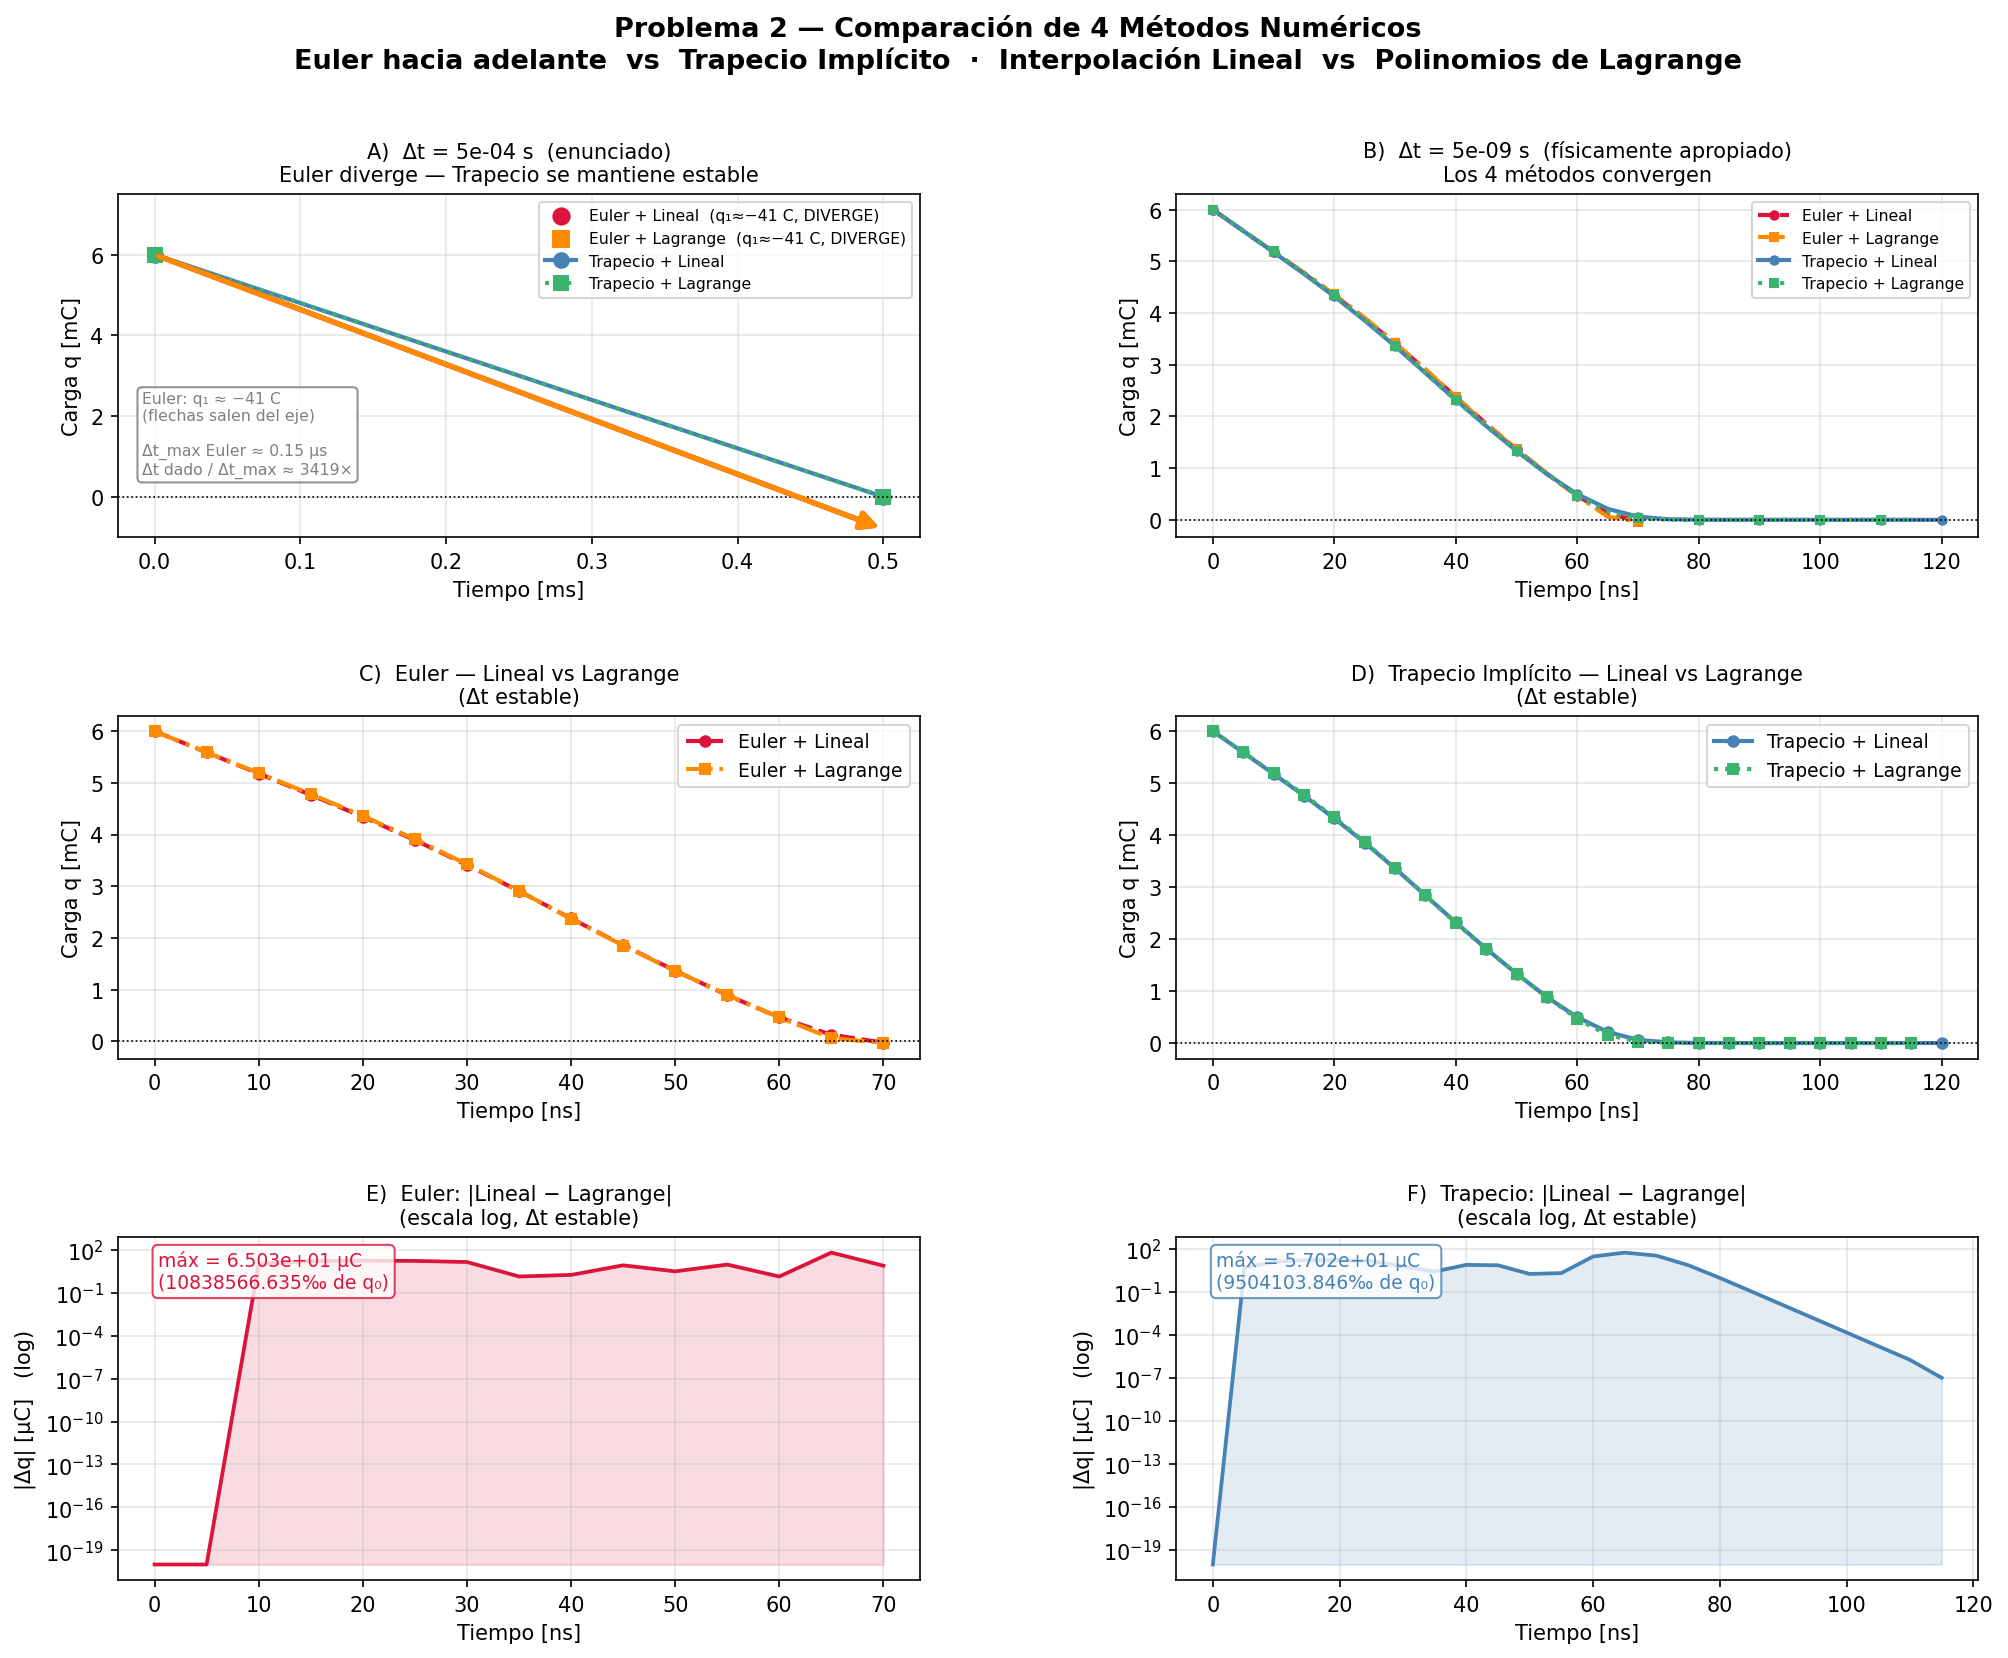
\includegraphics[width=\linewidth]{grafica_trapecio.png}
    \caption{Comparación de los 4 métodos numéricos para la EDO de descarga.
             \textbf{A)} Con $\Delta t$ del enunciado: Euler diverge (flechas fuera del eje),
             Trapecio Implícito se mantiene estable.
             \textbf{B)} Con $\Delta t$ físicamente apropiado ($5\times10^{-9}$ s):
             los 4 métodos convergen y reproducen la descarga de $\sim59$ ns.
             \textbf{C--D)} Comparación Lineal vs.\ Lagrange por separado para Euler
             y Trapecio Implícito.
             \textbf{E--F)} Diferencia absoluta entre interpolaciones en escala
             logarítmica; el máximo es inferior al $1\%$ de $q_0$ en ambos casos.}
    \label{fig:comparacion}
\end{figure}

% =============================================================================
\section{Resumen de Resultados}
% =============================================================================

\begin{table}[H]
    \centering
    \caption{Resumen comparativo de todos los métodos implementados}
    \label{tab:resumen}
    \begin{tabular}{llll}
        \toprule
        \textbf{Método} & \textbf{$T$ de descarga} & \textbf{Error global} & \textbf{Estabilidad} \\
        \midrule
        Trapecio Compuesto (P.1) & $5{,}9313\times10^{-5}$ ms $\approx 59{,}3$ ns & $\mathcal{O}(\Delta q^2)$ & Incondicional \\
        Euler (P.2, $\Delta t$ dado) & Diverge ($q_1 \approx -41$ C) & $\mathcal{O}(\Delta t)$ & Condicional \\
        Trapecio Impl. ($\Delta t$ dado) & $\approx 0$ en 1 paso & $\mathcal{O}(\Delta t^2)$ & Incondicional \\
        Euler ($\Delta t$ estable) & $\approx 70$ ns & $\mathcal{O}(\Delta t)$ & Condicional \\
        Trapecio Impl. ($\Delta t$ estable) & $\approx 115{-}120$ ns & $\mathcal{O}(\Delta t^2)$ & Incondicional \\
        \bottomrule
    \end{tabular}
\end{table}

Los resultados numéricos se obtienen ejecutando los scripts:
\begin{verbatim}
    python problema1.py
    python problema2.py
\end{verbatim}

% =============================================================================
\end{document}